\section{설치하기}\label{sec:install}

이 절에서는 \OCAML{}을 설치하는 방법을 각 플랫폼 별로 알아 봅니다. 자신이
사용할 플랫폼 외의 절은 보지 않아도 무방합니다.

\subsection{\LINUX{}}

\OCAML{}은 주로 \UNIX{} 대상으로 개발된 언어이며 설치 과정 또한 일반적인
\UNIX{} 프로그램의 방식을 따릅니다. 따라서 \UNIX{} 계열의 대표적인 운영체제인
\LINUX{}에서는 \OCAML{} 설치가 매우 간단합니다. 여기서는 여러
\LINUX{} 시스템 중에서 널리 쓰이는 \DEBIAN{} 계열의 시스템인 \UBUNTU{}를
대상으로 설치방법을 설명하겠습니다. 여타 \LINUX{} 시스템에서도 설치에 필요한
패키지명이 조금 다를 뿐 설치방법은 대동소이합니다.

\LINUX{}에서 \OCAML{}을 설치하는 방법은 세 가지가 있습니다. \LINUX{}
개발진이 제공하는 미리 컴파일된 바이너리 패키지를 설치하는 방법, \OCAML{}
소스를 직접 컴파일하는 방법, 그리고 \GODI{}라는 \OCAML{} 패키지 관리자를
설치하면서 자동으로 소스를 컴파일하는 방법. 아무래도 첫 번째 방법이 가장
쉽습니다만, 한 번쯤은 소스를 직접 컴파일 해보는 것도 경험상
좋습니다. 개인적으는 향후 패키지 관리에 유용한 세번째 방법, \GODI{}를 설치하는
것을 추천합니다.

\subsubsection{바이너리 패키지 설치}

바이너리 패키지 설치는 간단합니다. 일반적인 환경에서는 다음과 같이
\texttt{ocaml}과 \texttt{ocaml-native-compilers} 패키지를 설치하면 \OCAML{}
시스템 전부가 설치됩니다.

\begin{lstlisting}
$ ~sudo apt-get install ocaml ocaml-native-compilers~
\end{lstlisting}

\OCAML{} 부가 라이브러리 중 \GRAPHICS{} 라이브러리는 \XWIN{}\를
사용합니다. 따라서 텍스트 터미널만 운용하는 서버 환경인 경우 앞의 명령으로
\OCAML{}\을 설치하면 불필요한 패키지가 다수 설치될 수
있습니다. \GRAPHICS{} 라이브러리를 제외한 나머지 \OCAML{} 시스템을
설치하려면 \texttt{ocaml} 대신 \texttt{ocaml-base-nox} 패키지를 설치합니다.

\begin{lstlisting}
$ ~sudo apt-get install ocaml-base-nox ocaml-native-compilers~
\end{lstlisting}

\OCAML{} 실행파일은 \texttt{/usr/bin}, 라이브러리는 \texttt{/usr/lib/ocaml}
디렉토리에 설치됩니다. 다음 명령으로 설치된 시스템의 버전을
확인해 보세요.

\begin{lstlisting}
$ ~ocaml -version~
The Objective Caml toplevel, version 3.12.1
$ ~ocamlc -version~
3.12.1
$ ~ocamlopt -version~
3.12.1
\end{lstlisting}

\subsubsection{\OCAML{} 소스 컴파일}

\OCAML{}은 오픈소스 소프트웨어입니다. 따라서 소스를 받아 직접 컴파일하여
\OCAML{} 시스템을 구축할 수도 있습니다. 만일 \OCAML{}\을 \texttt{/usr/bin}이
아닌 다른 디렉토리에 설치하거나, 여러 버전의 \OCAML{}을 운용해야 한다면
바이너리 패키지 설치 대신 이 방법 (혹은 다음의 \GODI{} 설치)을 사용해야
합니다.

\OCAML{} 소스는 다음 웹사이트에서 받을 수 있습니다. 가장 맨 위의 ``Source
distribution'' 중 하나를 다운받으면 됩니다.

\begin{center}
\URL{http://caml.inria.fr/download.en.html}
\end{center}

우선 받은 파일의 압축을 풀고 디렉토리 안으로 이동합니다.

\begin{lstlisting}
$ ~tar xvfz ocaml-4.00.0.tar.gz~
...
$ ~cd ocaml-4.00.0~
\end{lstlisting}

디렉토리 안에 있는 \texttt{INSTALL} 파일에 컴파일 방법이 상세히 기술되어
있습니다. 문제가 발생하면 이 파일을 자세히 살펴보세요. 이후 컴파일은
\texttt{INSTALL} 파일 내용을 핵심 부분만 간추려서 진행하겠습니다.

\paragraph{사전 준비} 설치에 앞서 컴파일에 필요한 패키지를
설치합니다. 우선 \OCAML{} 일부는 \CC{}로 작성되었기 때문에 \CC{} 컴파일러와
컴파일에 쓰이는 \texttt{make}와 같은 도구가 필요합니다. 이러한 대부분의 도구는
\texttt{build-essential} 패키지를 설치하면 한 번에 설치됩니다.

\begin{lstlisting}
$ ~sudo apt-get install build-essential~
\end{lstlisting}

덧붙여 부가로 제공되는 \GRAPHICS{} 라이브러리를 같이 컴파일하려면
\texttt{lib-x11dev} 패키지를, \LABLTK{} 라이브러리를 컴파일하려면 \texttt{tk-dev}
또한 설치합니다.

\begin{lstlisting}
$ ~sudo apt-get install lib-x11dev tk-dev~
\end{lstlisting}

\paragraph{컴파일 설정} 컴파일에 앞서 컴파일 설정 스크립트인
\texttt{configure}\를 실행해야 합니다. 디폴트 디렉토리인 \texttt{/usr/local}
밑에 \OCAML{}을 설치하려면 별다른 옵션없이 스크립트를 그대로 수행하면 됩니다.

\begin{lstlisting}
$ ~./configure~
...
** Configuration summary **
...
** OCaml configuration completed successfully **
\end{lstlisting}

마지막 요약란에는 컴파일 시 사용될 옵션과 설치할 디렉토리, 같이 컴파일 할 부가
라이브러리에 관한 정보가 나옵니다.

만일 다른 디렉토리에 설치하길 원한다면 \texttt{--prefix} 옵션으로 디렉토리를
지정해 줘야 합니다.

\begin{lstlisting}
$ ~./configure --prefix /opt~
...
** Configuration summary **

Directories where OCaml will be installed:
        binaries.................. /opt/bin
        standard library.......... /opt/lib/ocaml
        manual pages.............. /opt/man (with extension .1)
...
\end{lstlisting}

여러 버전의 \OCAML{}\을 사용해야 하거나 나중에 \OCAML{}\을 삭제할 것이라면
\texttt{/usr/local} 대신 \texttt{/opt}와 같이 따로 떨어진 디렉토리에 설치하는
것도 좋은 방법입니다. 흔히 사용하는 방법은 \texttt{/opt/ocaml-4.00} 와 같은
디렉토리에 따로 설치하도록 설정하고, 그 디렉토리를 가리키는
\texttt{/opt/ocaml} 심볼릭 링크를 만드는 것입니다. 이렇게 해 놓으면 단순히
심볼릭 링크를 바꾸거나 원 디렉토리를 지우는 것으로 해당 \OCAML{}이 시스템에서
사라지게 할 수 있습니다.

\paragraph{컴파일} 이제 다음과 같이 \texttt{make}를 실행하여 \OCAML{}을 컴파일
합니다. 컴파일은 5분 이상은 소요되니 잠시만 쉬다가 오세요.

\begin{lstlisting}
$ ~make world.opt~
\end{lstlisting}

컴파일이 완료되면 만들어진 \OCAML{} 시스템을 설치해야 합니다. 다음 명령을
실행하면 설정 단계에서 지정한 디렉토리 밑의 \texttt{bin}, \texttt{lib/ocaml},
\texttt{man} 디렉토리에 실행파일, 라이브러리, 매뉴얼이 설치됩니다.

\begin{lstlisting}
$~ make install~
\end{lstlisting}

만일 설치 디렉토리가 \texttt{/usr/local}과 같은 시스템 디렉토리인
경우에는 권한이 없어 설치하지 못할 수 있습니다. 이 경우에는 다음과 같이 관리자
권한으로 설치합니다.

\begin{lstlisting}
$ ~sudo make install~
\end{lstlisting}

마지막으로 \texttt{\~{}/.bashrc}와 같은 쉘 설정 파일에 다음과 같은 설치 디렉토리
설정을 추가합니다. 여기서는 설치 디렉토리가 \texttt{/usr/local}이라
가정합니다. 변경된 설정 파일은 쉘을 재시작해야 적용됩니다.

\begin{lstlisting}
~export PATH=/usr/local/bin:$PATH
export MANPATH=/usr/local/man:$MANPATH~
\end{lstlisting}

이제 다음 명령으로 설치된 \OCAML{} 버전을 확인해 볼 수 있습니다.

\begin{lstlisting}
$ ~ocaml -version~
The Objective Caml toplevel, version 4.00.0
$ ~ocamlc -version~
4.00.0
$ ~ocamlopt -version~
4.00.0
\end{lstlisting}


\subsubsection{\GODI{} 설치}

\TODO{Linux GODI 설치}

\subsection{\MAC{}}

\TODO{Mac 시스템에 설치하기}


\subsection{\WINDOWS{}}

슬프게도 \OCAML{}은 \WINDOWS{}와 사이가 썩 좋지 않습니다. 기본적으로
\OCAML{}은 \UNIX{} 환경을 대상으로 개발되고 있기 때문에, \UNIX{}와 많은 차이가
있는 \WINDOWS{}에서의 \OCAML{} 작업은 그렇게 매끄럽지가 않아요. 일부
라이브러리는 \WINDOWS{} 용으로 아예 구현이 되지 않을 정도입니다.

하지만 현재는 많은 오픈소스 개발자의 노력 덕분에 예전보다 \WINDOWS{}에서의
작업이 많이 수월해진 편입니다. 일단 \CYGWIN{}이라고 하는 \UNIX{} 환경을
흉내내는 시스템과 \MINGW{}라고 하는 \WINDOWS{} 용 \CC{} 컴파일러가 많이
개선되었습니다. 그리고 \textsf{flexdll}과 같은 동적 라이브러리 연결 도구 또한
생겨났고, 이러한 환경을 한 번에 설치해 주는 인스톨러 또한 만들어 졌습니다.

여기서는 \OCAML{} 공식 설치 프로그램를 가지고 \OCAML{}을 설치하는 과정을
설명합니다. \LINUX{}, \MAC{} 시스템에서의 설치와 달리, \WINDOWS{} 시스템에서
소스를 직접 컴파일 하기에는 고려해야 할 점이 너무 많으므로 여기서는 소스
컴파일 방법에 대해서는 설명하지 않습니다. \CYGWIN{} 패키지를 설치하는 방법도
있으나, 이렇게 되면 \OCAML{} 프로그램이 \CYGWIN{} 라이브러리를 거쳐서 동작하기
때문에 느려지므로 이 역시 설명하지 않습니다.

\subsubsection{설치 프로그램으로 설치}

우리가 사용할 설치 프로그램은 여러 소프트웨어를 자동으로 설치합니다. 우선
\OCAML{}을 설치하며, \OCAML{} 라이브러리를 관리하는 \FINDLIB{}과 동적
라이브러리(DLL) 생성을 도와주는 \textsf{flexdll} 또한 설치합니다. 그리고
사용자 선택에 따라서 \EMACS{}와 \OCAML{} 기본 \EMACS{} 플러그인, \TK{}
라이브러리를 위한 \textsf{ActiveTCL} 또한 설치합니다. 마지막으로 원할한
\OCAML{} 개발 환경을 위해 \CYGWIN{}과 개발에 필요한 패키지를 설치합니다.

앞에서 살펴본 대로 설치 프로그램은 \CYGWIN{} 시스템을 알아서 다운받은 후 설치하는
기능을 제공합니다. 하지만 \CYGWIN{} 설치를 한 번쯤 직접 해보는 것도
중요하므로, 여기서는 일단 설치 프로그램에 앞서 우리가 직접 \CYGWIN{}을 먼저
설치하도록 하겠습니다.

\CYGWIN{}을 이미 설치한 상태라면 다음 \textbf{\CYGWIN{} 설치} 부분은 넘어가도
좋습니다. 단 \CYGWIN{}을 매우 오래전에 설치했다면 넘어가지 말고 다시 한 번
설치하여 기존 시스템을 업데이트 하는 것이 좋습니다.

\paragraph{\CYGWIN{} 설치} \CYGWIN{} 설치 프로그램은 다음 주소에서
다운로드 받을 수 있습니다.

\begin{center}
\URL{http://cygwin.com}
\end{center}

``Current Cygwin DLL version'' 부분에 있는 ``setup.exe'' 링크를 클릭하면
됩니다. 설치하는 방법은 다음과 같습니다.

\begin{itemize}
\item 받은 \texttt{setup.exe} 파일을 더블 클릭하면 설치 프로그램 화면이
  열립니다. ``다음''을 클릭하세요.
\item 이제 무엇을 할 것인지 선택하는 화면이 뜨는데, 이미 선택되어 있을
  ``Install from Internet''을 선택하고 다시 ``다음''을 클릭합니다.
\item \CYGWIN{}을 설치할 디렉토리를 입력하는 창이 열립니다. 되도록 미리
  지정되어 있는 \texttt{C:\textbackslash cygwin} 디렉토리를 사용하는 것이
  좋습니다. 만일 부득이하게 다른 디렉토리를 지정해야 한다면 디렉토리 이름
  사이에 공백이 없도록 하세요. 디렉토리를 지정하였다면 ``다음''을 클릭합니다.
\item 이번에는 \CYGWIN{}이 \UNIX{} 프로그램을 설치하기 전에 다운로드 할
  디렉토리를 지정합니다. 이 디렉토리는 실제 \UNIX{} 프로그램이 설치되는
  장소와는 관련이 없습니다. 실제로 설치후에는 디렉토리를 지워도
  무방합니다. 아무 곳이나 지정한 후 ``다음''을 클릭합니다.
\item 인터넷 접속 방식을 선택합니다. 프록시를 쓰지 않는다면 ``다음''을
  클릭합니다.
\item 이제 설치 프로그램은 \CYGWIN{} 패키지를 보유하고 있는 미러 사이트 목록을
  받아온 후 보여줍니다. 목록 중에서 가장 빠를 것 같은 곳을 하나
  선택하고 ``다음''을 클릭합니다.
\item 설치 프로그램은 미러 사이트에서 프로그램 목록을 받습니다. 이후에 ``Setup
  alert''이 뜰 수 있는데, 이는 아주 예전 버전의 \CYGWIN{}을 설치한 상태라면
  업그레이드 전에 홈페이지에서 유의사항을 확인하라는 의미입니다. ``확인''을
  클릭하고 다음으로 넘어갑니다.
\item 여기까지 진행하였다면 설치할 \CYGWIN{} 패키지를 선택하는 그림
  \ref{fig:cygwin} 창이 열립니다.
  \begin{figure}[t]
    \centering
    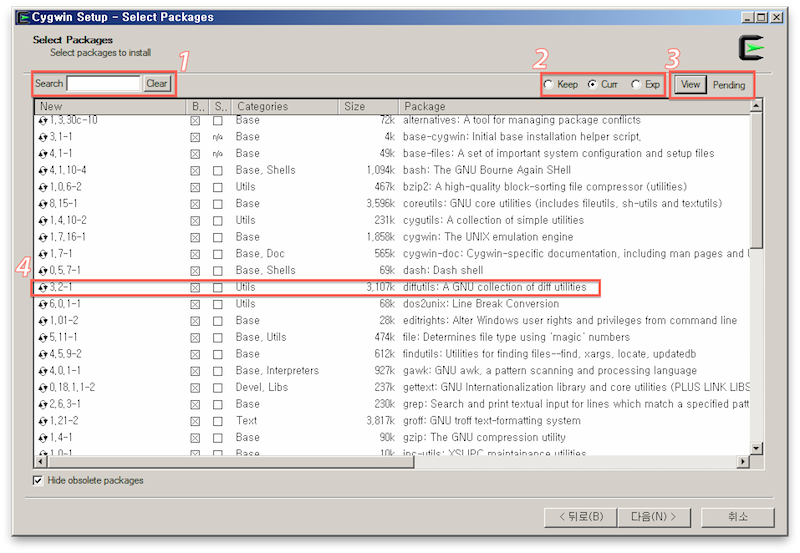
\includegraphics[width=0.9\textwidth]{img/cygwin.png}
    \label{fig:cygwin}
    \caption{설치할 \CYGWIN{} 패키지 선택}
  \end{figure}
  가운데에는 많은 \CYGWIN{} 패키지 목록이 보입니다. 각 부분의 의미하는 바는
  다음과 같습니다.
  \begin{enumerate}
  \item 검색란입니다. 설치할 패키지 이름을 입력하면 패키지 목록이 걸러집니다.
  \item 이 버튼 중 하나를 클릭하면 패키지를 자동으로 선택합니다. ``Keep''은
    현재 \CYGWIN{} 시스템에 설치된 패키지를 그대로 유지한다는 의미입니다. 이를
    클릭하면 새로 패키지를 설치하거나 삭제하려고 선택한 사항은 모두
    취소됩니다. 그 옆의 ``Curr''은 현재 설치된 패키지 중 안정 버전으로 업데이트
    할 수 있는 것을 모두 선택하라는 의미입니다. ``Exp''은 ``Curr''과 비슷하지만
    단 안전성이 고려되지 않은 실험 버전의 패키지도 고려합니다.\footnote{여기서
      실험 버전이란 원 프로그램 개발 측(upstream)에서 실험 중이라는 것이
      아니라, 그 프로그램이 \CYGWIN{} 시스템에서 제대로 동작하는지를 \CYGWIN{}
      개발진에서 실험 중에 있다는 의미입니다. 따라서 실험 버전이어도 그것이 원
      프로그램의 최신 버전보다 옛 버전일 수도 있습니다.}
  \item 패키지 목록 형식을 지정하는 버튼입니다. 버튼을 누를 때마다
    가운데 패키지 목록이 바뀝니다. ``Pending''은 현재 설치 대상으로 지정된
    패키지만을 보여 줍니다. 설치할 패키지를 아무것도 지정하지 않더라도
    업데이트 혹은 \CYGWIN{}에 필요한 패키지가 자동으로 지정되어 있을 수도
    있습니다. ``Up To Date''는 현재 설치된 패키지 중 최신 버전의 패키지를,
    ``Not Installed''는 아직 설치되지 않은 패키지만을 보여
    줍니다. ``Category''는 패키지 목록 전체를 패키지 종류별로 분류하여,
    ``Full''은 일렬로 나열하여 보여줍니다.
  \item 패키지의 정보입니다. 맨 앞은 이번 설치 과정에서 해당 패키지를 어떻게
    다룰지를 설정하는 란입니다. 클릭하면 패키지를 설치 혹은 제거하도록 지정할
    수 있습니다. ``Skip''은 이 패키지를 설치하지 않을 것임을 나타냅니다. 그 외
    숫자는 설치할 패키지 버전 정보를 나타냅니다. 여러 버전이 있다면 계속
    클릭할 때마다 버전이 바뀝니다. 중간의 ``B'' 란은 바이너리 설치 여부, ``S''
    란은 소스 코드 설치 여부입니다. 이 항목은 크게 신경쓰지 않아도 됩니다.
  \end{enumerate}
\item 이제 패키지 설치란에서 \OCAML{} 설치에 필요한 패키지를
  설치합시다. 필요한 패키지는 \texttt{curl}, \texttt{make},
  \texttt{mingw64-i686-gcc-g++}, \texttt{mingw64-i686-gcc}, \texttt{patch},
  \texttt{rlwrap}, \texttt{libreadline7} (없다면 \texttt{libreadline6}), \texttt{diffutils} 입니다. 각
  패키지를 찾아서 맨 왼쪽 ``Skip''을 클릭, 최신 버전을 설치하도록
  지정합니다.
\item 설치할 패키지를 지정하였으면 ``다음''을 클릭합니다. 설치에 앞서 선택한
  패키지가 의존하는 다른 패키지도 같이 설치할 것인지 물어볼 수 있는데,
  여기서도 ``다음''을 클릭합니다. 그러면 이제 설치가 진행됩니다. 잠시 쉬다
  오세요.
\item 설치가 끝나면 바로가기를 등록할 것인지를 물어봅니다. 처음 설치하는
  것이라면 ``Add icon to Start menu''는 선택해 둡니다. 적절히 지정하고
  ``마침''을 클릭합니다.
\end{itemize}

참고로 설치가 끝나고 난 후 \texttt{setup.exe} 파일은 삭제하여도
무방합니다. 하지만 차후에 추가로 패키지를 설치해야 하는 경우에 다시 이 파일을
실행해야 하므로, 되도록 삭제하지 말고 적절한 디렉토리에 보관해 두세요. 추천하는
방법은 \texttt{setup.exe} 파일을 \CYGWIN{} 설치 디렉토리 안에 넣어두고
바로가기를 만들어 두는 것입니다.

이제 \CYGWIN{} 시스템을 사용할 수 있습니다. 바로가기를 등록해 두었다면,
시작 메뉴 내 ``Cygwin'' 프로그램 폴더 안에 ``Cygwin Terminal'' 아이콘이
추가되었을 것입니다. 이것을 클릭하면 \CYGWIN{} 시스템에서 동작하는 쉘 터미널
실행할 수 있고, 여기서 \UNIX{} 명령을 사용하면 됩니다. 만일 현재 자신이
\WINDOWS{} 어느 폴더에 있는 것인지 알고 싶다면 다음 명령을 입력하세요.

\begin{lstlisting}
$ ~explorer.exe .~
\end{lstlisting}

\CYGWIN{} 설치가 끝났으니 이제 본격적으로 \OCAML{}을 설치해 봅시다.

\paragraph{\OCAML{} 설치} \OCAML{} 설치 프로그램은 다음 주소에서
내려받을 수 있습니다. (\OCAML{} 공식 웹사이트 다운로드 페이지의 ``Binary
distributions for Microsoft Windows'' 중 ``Self installer''가 이곳에 연결됩니다).

\begin{center}
  \URL{http://protz.github.com/ocaml-installer/}
\end{center}

가운데 ``Installer for OCaml'' 링크를 내려받으면 됩니다. 내려받은 파일을
실행하여 다음과 같이 설치를 진행합니다.

\begin{itemize}
\item 설치 프로그램을 실행하면 귀여운$^?$ 낙타가 우리를 반겨줍니다. ``Next''를
  클릭합니다.
\item 설치할 프로그램 폴더를 지정하고 ``Next''를 클릭합니다.
\item \OCAML{} 라이센스를 보여줍니다. ``Next''를 클릭합니다.
\item 이제 설치할 프로그램을 선택하는 창이 열립니다. 당연히 ``OCaml''은
  선택. ``ActiveTCL''은 부가 라이브러리 중 하나인 \LABLTK{}를
  사용하는데 쓰입니다. 선택하지 않아도 무방합니다. 다음의 ``Emacs''는
  편집기인데, 일단은 선택하지 마세요. ``Emacs'' 설치 방법은
  \ref{sec:ide}절에서 따로 다룹니다. 그리고 앞에서 이미 \CYGWIN{}을
  설치했으므로 마지막 ``Cygwin''은 선택을 해제해야 합니다. 결정하였으면
  ``Next''를 클릭합니다.
\item \OCAML{} 설치 폴더를 지정합니다. 되도록 미리 주어지는
  \texttt{C:\textbackslash OCaml}을 그대로 사용하세요. 만일 다른 곳에 설치해야
  한다면 폴더명 사이에 공백이 들어가지 않도록 유의합니다. 정했으면
  ``Install''을 클릭해서 설치를 시작합니다.
\end{itemize}

설치가 모두 끝나면 \CYGWIN{} 터미널을 열어서 다음과 같이 설치한 \OCAML{}
버전을 확인해 볼 수 있습니다.

\begin{lstlisting}
$ ~ocaml -version~
The Objective Caml toplevel, version 4.00.0
$ ~ocamlc -version~
4.00.0
$ ~ocamlopt -version~
4.00.0
\end{lstlisting}

시작 메뉴 안에는 \textsf{OCamlWin}이라는 프로그램이 있는데, 이를 실행하면
\OCAML{} 탑레벨을 터미널 밖에서도 쓸 수 있습니다.

\subsubsection{문제 해결}

\WINDOWS{} 환경에서 발생할 수 있는 \OCAML{} 문제를 해결하는 방법에 대해
설명합니다.

\begin{itemize}
\item \OCAML{} 실행 시 ``\texttt{Fatal error: cannot open pervasives.cmi}'' 와
  같은 오류 발생 -- \OCAML{} 표준 라이브러리의 위치를 찾지 못하는 경우입니다.
  우선 터미널에서 다음 명령을 입력으로 \OCAML{}이 사용하는 표준 라이브러리
  폴더를 확인합니다.

  \begin{lstlisting}
$ ~ocamlc -where~
c:\ocaml-3.11\lib
  \end{lstlisting}

  이 명령의 결과는 설치 과정에서 지정한 폴더 내 \texttt{lib} 폴더의 경로이어야
  합니다. (미리 지정된 폴더를 사용한 경우,
  \texttt{C:\textbackslash{}OCaml\textbackslash{}lib}). 잘못된 경로가
  출력된다면 \texttt{OCAMLLIB} 환경변수를 확인해 봐야 합니다. 우선 ``제어판'' 내
  ``시스템''을 열고 ``고급 시스템 설정''을 클릭해서 ``시스템 속성'' 창을
  엽니다. (\textsf{Windows XP}의 경우 ``시스템''만 열면 바로 열림). 여기서
  ``고급'' 탭의 ``환경 변수''를 클릭하면 시스템에 정의된 환경 변수를 찾아볼 수
  있습니다. 우리가 사용한 설치 프로그램으로 \OCAML{}을 설치하면
  \texttt{OCAMLLIB}과 같은 환경 변수는 설정할 필요없습니다. 사용자 변수,
  시스템 변수 목록에서 \texttt{OCAMLLIB}이 보이면 삭제하고 ``확인''
  클릭합니다. 그리고 나서 환경 변수 적용을 위해 터미널을 재시작해서 다시
  \OCAML{}을 실행하면 됩니다.

  만일 이 방법으로도 문제가 계속된다면 표준 라이브러리 파일에 문제가 생긴 것일 수
  있습니다. 설치 과정에서 지정한 폴더 내 \texttt{lib} 폴더가 제대로 있는지
  확인하고, \OCAML{}을 삭제한 후 재설치하세요.
\end{itemize}

%%% Local Variables: 
%%% mode: latex
%%% TeX-master: "master"
%%% End: 
